\doublespacing % Do not change - required

\chapter{ Methodology}
\label{ch3}

%%%%%%%%%%%%%%%%%%%%%%%%%%%%%%%%%%%%%%%
% IMPORTANT
\begin{spacing}{1} %THESE FOUR
\minitoc % LINES MUST APPEAR IN
\end{spacing} % EVERY
\thesisspacing % CHAPTER
% COPY THEM IN ANY NEW CHAPTER
%%%%%%%%%%%%%%%%%%%%%%%%%%%%%%%%%%%%%%%



\section{Programmable Logic Controller (PLC)}

PLC is a control device that enables processes to be managed safely, efficiently and flexibly in industrial automation systems. Dick Morley is an electrical engineer known as the father of PLC. Morley is the founder and president of Bedford Associates, where he created Modicon in 1968. PLC was first used in General Motors factories. PLCs, which can control automation elements such as sensors, buttons, motors, relays and contactors through input-output modules, offer advantages such as taking up less space, having fewer failures and performing faster processes compared to classic relay systems. For these reasons, they have replaced traditional relay systems over time.

\begin{figure}[H]
    \centering
    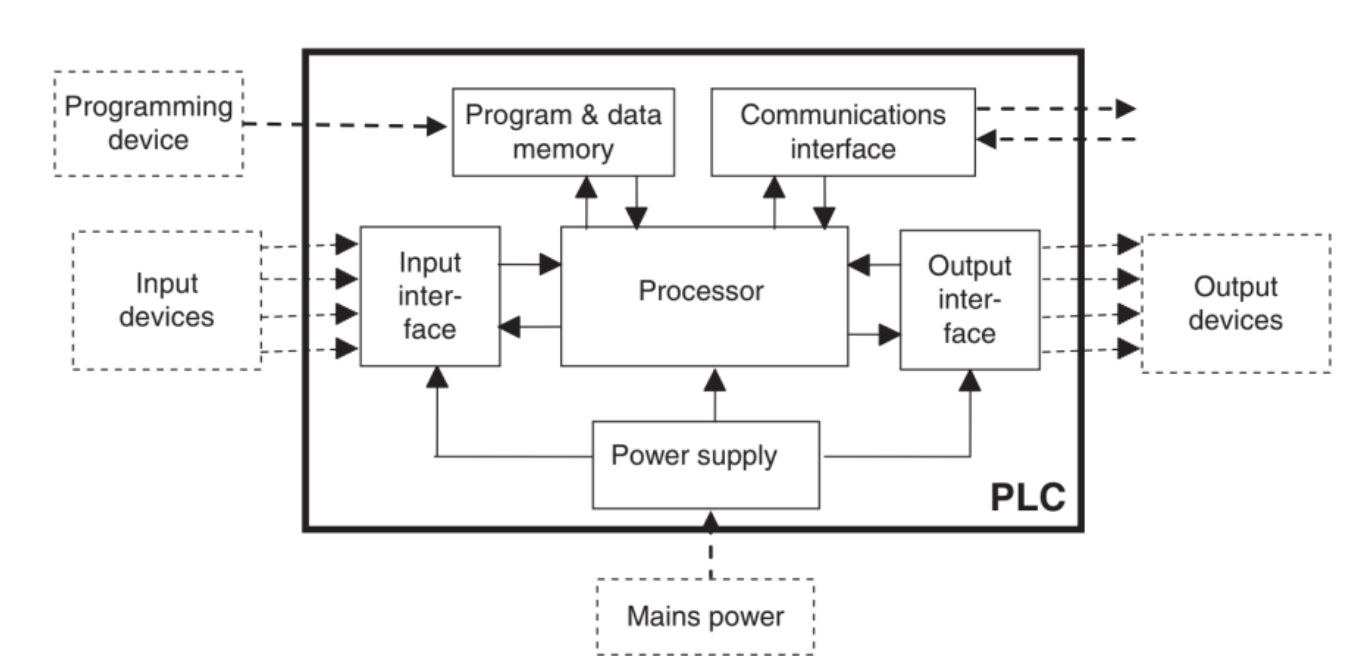
\includegraphics[width=0.8\columnwidth]{imgs/The PLC system.png}
    \caption[Short description for list of figures]{The PLC system }
    \label{fig-magnitude}
    \end{figure}%


    The basic components of the PLC include the Central Processing Unit (CPU), Memory Unit, Input-Output (I/O) Unit, Signal Compatibility Circuits and Expansion Modules. The CPU is the management center of the system and performs arithmetic and logical operations by processing the signals it receives from the input units, then controls the automation processes by transmitting the appropriate commands to the output units. Basic functions such as Timer, Counter and Comparator are operated within the CPU in order to perform the specified process flows. The Memory Unit, which determines the operating logic of the CPU, allows the storage of program codes and process data. In this context, RAM stores temporary data, while ROM and EPROM ensure that the program is protected in the event of a power outage and rewritten when necessary. This structure increases the flexibility and long-term operational sustainability of the system. The Input-Output (I/O) Unit is the main component that enables the PLC to exchange data with the physical world. Input modules receive analog or digital signals from sensors, buttons, and switches and convert them into digital data formats that the CPU can process. Output modules convert the commands processed by the CPU into appropriate electrical signals that will operate actuators such as motors, relays, and solenoid valves. Signal Compatibility Circuits in the system regulate the voltage levels of signals coming from/going to input and output units, provide protection, and enable the PLC to communicate safely with different system components.

    \begin{figure}[H]
        \centering
        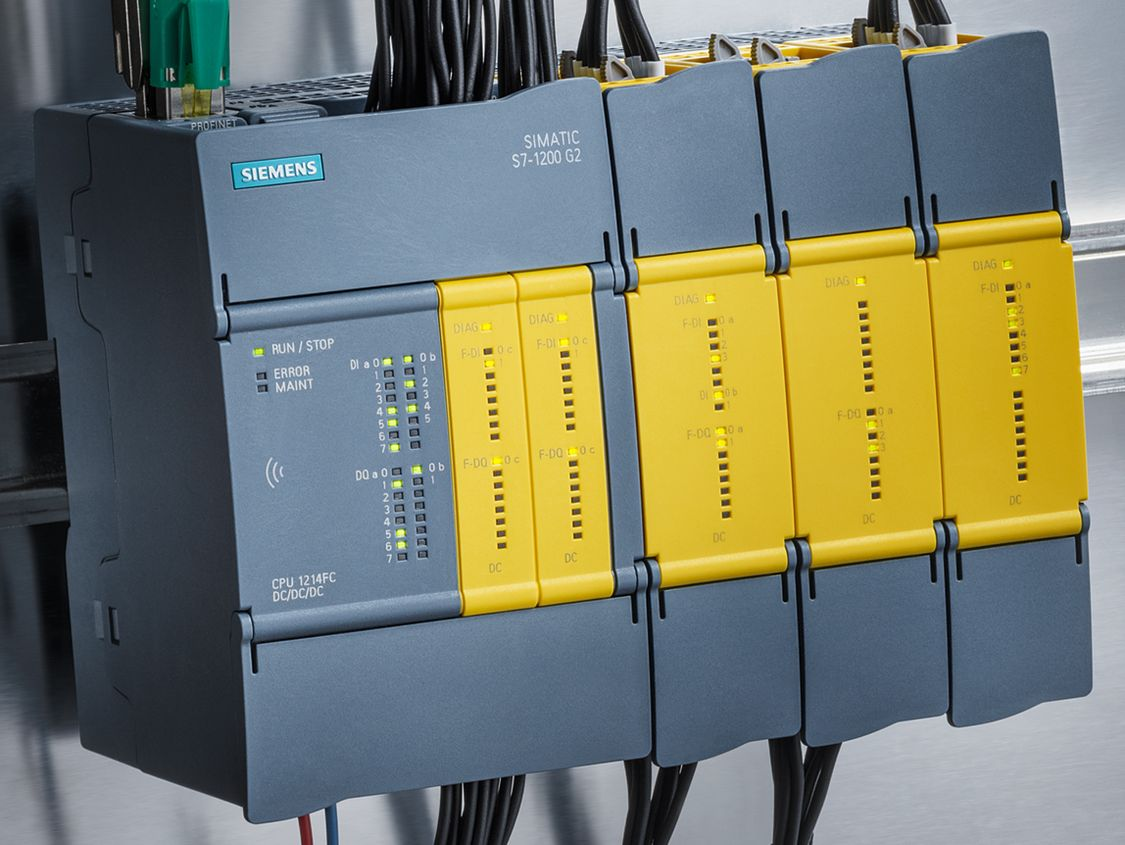
\includegraphics[width=0.8\columnwidth]{imgs/SIMATIC-S7-1200-G2.jpg}
        \caption[Short description for list of figures]{SIMATIC-S71200 }
        \label{fig-magnitude}
        \end{figure}%   
    
        In our study, Siemens S7-1200 series PLC model was preferred. Siemens S7-1200 is a common programmable logic controller (PLC) model that offers expandability thanks to its modular structure, operates with 24V DC supply voltage and provides high-speed switching capability via digital input-output modules and transistor outputs. Its compatibility with communication protocols such as Modbus and Profinet facilitates integration with different automation systems; and thanks to its high resistance to harsh environmental conditions, it offers a wide range of applications from industrial facilities to energy management systems. The CPU 1214C model of the series offers a reliable and scalable control solution in industrial areas such as automatic production lines, process control systems, building automation and energy management with its fast processing capacity, comprehensive communication protocol support and robust structure; It is effectively used in applications requiring high performance.



       
\section{Modbus}

Modbus is one of the oldest and most common protocols that provide communication between PLCs and other industrial devices. It was developed by Modicon in 1978 and over time it has become a standard communication method that provides data transfer and information exchange between PLC systems.

Modbus, which works with the master-slave model, has been divided into different versions such as Modbus RTU and Modbus TCP over time. While Modbus RTU is based on serial communication, Modbus TCP is TCP/IP based. While the PDU (Protocol Data Unit) is fixed in data transmission and works independently of the lower layer, the content of the Modbus ADU (Application Data Unit) changes according to the type of protocol used. Figure 5 shows the structure of the Modbus ADU and Modbus TCP/IP ADU data packets. Modbus RTU and Modbus ASCII use serial communication (RS-232, RS-485) and the ADU structure consists of Address (1 byte), Function Code (1 byte), Data (n bytes) and Error Check (CRC, 2 bytes) components. Modbus TCP/IP communicates over Ethernet and uses MBAP Header (7 bytes) instead of CRC for error checking. The ADU structure consists of MBAP Header (7 bytes), Function Code (1 byte) and Data (n bytes) components. PDU (Function Code + Data) is common in both structures. Modbus RTU/ASCII transmits data over serial ports (RS-232, RS-485), while Modbus TCP/IP transmits data over the Ethernet network, but both systems use the same data processing logic. 

\begin{figure}[H]
    \centering
    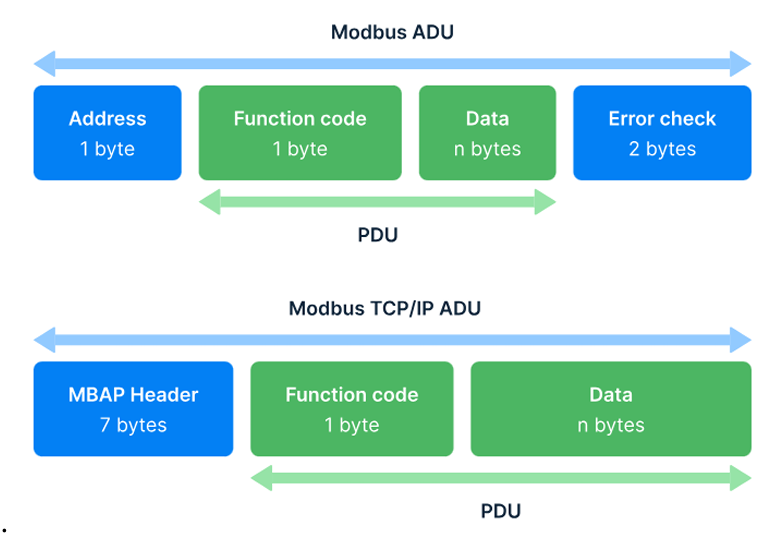
\includegraphics[width=0.8\columnwidth]{imgs/PDU and ADU.png}
    \caption[Short description for list of figures]{PDU and ADU}
    \label{fig-magnitude}
    \end{figure}%

    The Modbus communication structure consists of two main components: the communication layer and the physical layer. The most commonly used methods are Modbus ASCII, Modbus RTU and Modbus TCP/IP. In the physical layer, communication is provided via RS232, RS485, USB and CAN connections, while Ethernet is used in TCP/IP-based communications. The function code (1 byte) in the PDU (Protocol Data Unit) determines the operating mode of the devices, while the data field contains the request and response parameters between the master and slave devices.
    The Modbus message structure consists of the device address, function code, data field and error control mechanisms. The master device expects an immediate response to the commands it sends; if no response is received, it repeats the process and uses timing and error control mechanisms to ensure communication reliability. While Modbus allows flexible parameter configurations in some systems, fixed settings that cannot be changed by the user are used in other systems. Although Modbus is slower than other communication protocols, it is widely preferred in the industry due to its wide manufacturer support and flexible structure.
    



    \medskip

    \section{Energy Tracking}

    Energy monitoring systems are automation and control solutions developed to ensure effective control of energy consumption, increase energy efficiency and continuous monitoring of energy quality. These systems provide a wide data collection and evaluation infrastructure consisting of measurement devices, communication protocols and analysis software.
Energy monitoring systems ensure the healthy operation and management of production, transmission and distribution points in electrical facilities. These systems allow rapid detection and intervention of faults occurring in energy lines.
Energy monitoring systems perform critical functions in energy management and optimization processes. Thanks to the real-time monitoring feature, electrical parameters such as voltage, current, power and frequency are continuously monitored and analyzed.
In addition, remote control capability enables remote monitoring and control of energy systems via communication protocols. This feature provides ease of management, especially in energy systems spread over large areas. The energy efficiency and saving function allows the determination of unnecessary energy use and optimization of costs by analyzing consumption data. In addition, the harmonic and quality analysis feature of the system allows the detection of harmonics and other fluctuations that deteriorate energy quality. Thus, corrective measures are taken to improve energy quality and ensure system reliability. All these functions make energy monitoring systems an indispensable tool for modern energy management.



\begin{figure}[H]
    \centering
    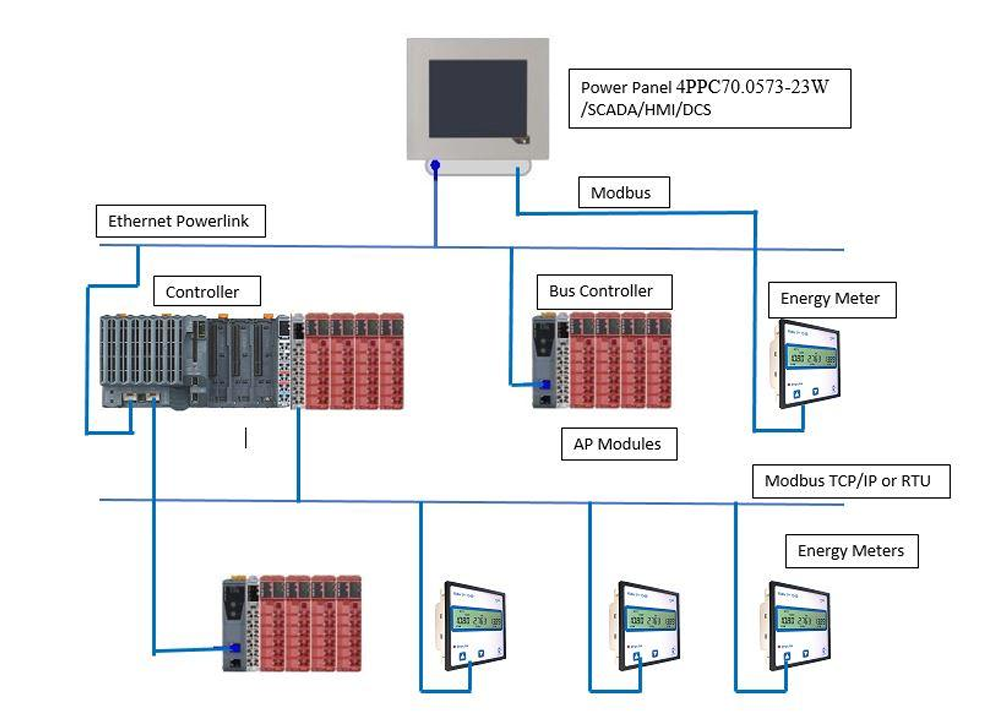
\includegraphics[width=0.8\columnwidth]{imgs/System Architecture of Energy Monitoring System.png}
    \caption[Short description for list of figures]{System Architecture of Energy Monitoring System }
    \label{fig-magnitude}
    \end{figure}%


    Energy monitoring systems are critical for monitoring energy consumption, increasing energy efficiency and ensuring energy quality. These systems help businesses reduce energy costs and provide sustainable energy management. Especially thanks to modern automation systems and communication technologies, energy monitoring systems have wider application areas.

    \medskip

    \subsection{Communication Protocols}  

    In energy monitoring systems, data transfer between devices is provided through communication protocols, and these protocols allow for secure, fast and uninterrupted data transmission. Modbus is the most widely used serial communication protocol in industrial automation systems. It provides a reliable communication infrastructure in energy monitoring systems by facilitating data transfer between devices such as PLCs and analyzers. The IEC 60870-5-101 protocol was specifically developed to ensure data security in critical energy infrastructures. It contributes to the continuous monitoring of energy systems by establishing secure communication between remote terminal units and smart electronic devices.


    \begin{figure}[H]
    \centering
    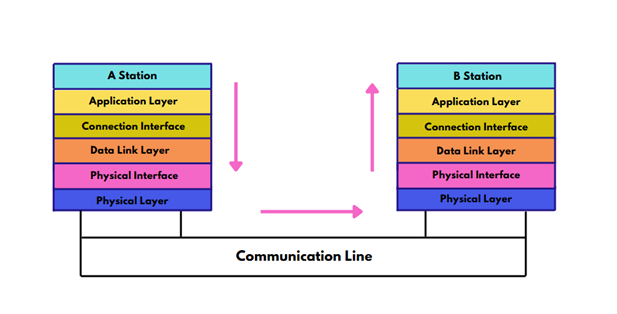
\includegraphics[width=0.8\columnwidth]{imgs/IEC 60870-5-101 Enhanced Performance Architecture Model.png}
    \caption[Short description for list of figures]{IEC 60870-5-101 Enhanced Performance Architecture Model }
    \label{fig-magnitude}
    \end{figure}%

    Wireless communication technologies such as ZigBee and Wi-Fi are frequently preferred in modern applications such as smart buildings and distributed energy production systems. These protocols have an important place in systems requiring wireless data transfer by offering low energy consumption and flexible connectivity. All these protocols provide uninterrupted data flow in energy monitoring systems, making energy management and analysis processes more reliable and efficient.



\medskip


\section{Modeling Motor}
This study aims to optimize energy consumption. The main energy-consuming components of the system are the conveyor systems and industrial robot arms in the production line. These two elements are directly connected to the drive systems, namely direct current (DC) motors, which convert electrical energy into mechanical energy in order to provide mechanical movement. Therefore, a large part of the total energy consumption is realized through these motors. In this context, a detailed examination of the operating characteristics of the motors in question and the regulation of their controllable parameters with the help of appropriate algorithms are of critical importance in terms of energy efficiency.

Within the scope of the project, the aim is to analyze the motor behavior by performing mathematical modeling of the DC motors used in the system.
The dynamic model of a typical DC motor is obtained by combining both electrical and mechanical subsystems.
In this context, in this project, we are trying to provide energy optimization by controlling these DC motors. The modeling of a DC motor is given below:

\begin{figure}[H]
    \centering
    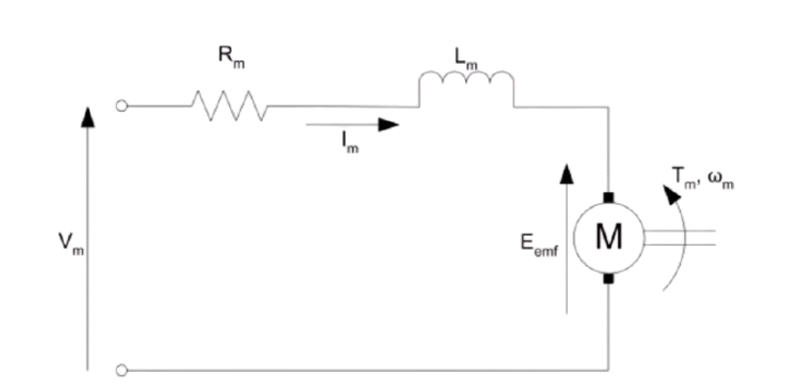
\includegraphics[width=0.8\columnwidth]{imgs/DC motor circuit.png}
    \caption[Short description for list of figures]{The circuit of DC motor }
    \label{fig-magnitude}
    \end{figure}%

    The stages of obtaining the transfer function of a DC electric motor are shown below:
    \begin{equation}
        V_m(t) = R_m I_m(t) + L_m \frac{d I_m(t)}{dt} + E_{emf} = 0
        \label{eq:dc_motor_voltage}
        \end{equation}

    The feedback voltage can be expressed as follows: 
        \begin{equation}
            E_{emf} = K_b W_m(t)
            \label{eqfeedback_voltage }
            \end{equation}

    The torque expression can be expressed as follows: 
            \begin{equation}
                T_m(t) = K_t I_m(t)
                \label{eq:torque_expression }
                \end{equation}

    The equivalent of torque in terms of viscosity and inertia is as follows:
            \begin{equation}
                T_m(t) = J_m \frac{d W_m(t)}{dt} + B_m W_m(t)
                \label{eq:mechanical_dynamics}
                \end{equation}
        

    Angular velocity equals the derivative of angular displacement:
            \begin{equation}
               W_m(t) = \frac{d \theta(t)}{dt}
                \label{eq:angular_velocity}
                \end{equation}
        

    If the voltage \( V_m(t) \) and torque \( T_m(t) \) expressed above are expressed in the frequency domain:
 
            \begin{equation}
                V_m(s) = R_m I_m(s) + L_m s I_m(s) + K_b W_m(s)
                \label{eq:voltage_laplace}
                \end{equation}
        
                \begin{equation}
                    T_m(s) = K_t I_m(s)
                    \label{eq:torque_current_laplace}
                    \end{equation}
                    
                \begin{equation}
                    T_m(s) = J_m s W_m(s) + B_m W_m(s)
                    \label{eq:mechanical_laplace}
                    \end{equation}
                        

    If \( K_t I_m(s) \) is substituted for the torque expression 

                \begin{equation}
                    K_t I_m(s) = J_m  W_m(s) + B_m W_m(s)
                    \label{eq:substituted_torque}
                    \end{equation}
        

    If the angular velocity is left alone, it is obtained as follows: 
    \begin{equation}
        W_m(s) = \frac{K_t I_m(s)}{J_m s + B_m}
        \label{eq:omega_from_current}
        \end{equation}
        
        If the angular velocity expression is substituted in equation 3.6, the voltage expression becomes 
        as follows: 

                \begin{equation}
                     V_m(s) = R_m I_m(s) + L_m s I_m(s) + K_b \left( \frac{K_t I_m(s)}{J_m s + B_m} \right)
                    \label{eq:vm_substitution_step1}
                    \end{equation}
        
                    \begin{equation}
                        V_m(s) = \left( R_m + L_m s + \frac{K_b K_t}{J_m s + B_m} \right) I_m(s)
                        \label{eq:vm_substitution_step2}
                        \end{equation}
    
    If the current expression is left alone, the following equation is obtained:

                \begin{equation}
                    I_m(s) = \frac{V_m(s)}{R_m + L_m s + \frac{K_b K_t}{J_m s + B_m}}
                    \label{eq:current_expression}
                    \end{equation}
        
    Earlier we stated that the angular velocity is:

    \begin{equation}
        W_m(s) = \frac{d \theta_m(s)}{ds}
        \label{eq:angular_velocity_laplace}
        \end{equation}
        
        Here the angular displacement, left alone, is equal to:
        
        \begin{equation}
            \theta_m(s) = \frac{W_m(s)}{s}
            \label{eq:angular_displacement_laplace}
            \end{equation}
            
            If the angular velocity is replaced by the expression in Equation 3.10 in the angle expression in 
Equation 3.15, the angular displacement is obtained as follows: 

\begin{equation}
    \theta_m(s) = \frac{K_t I_m(s)}{J_m s^2 + B_m s}
    \label{eq:theta_current_relation}
    \end{equation}

    
    If the expression for \( I_m(s) \) in Equation 3.16 is replaced by the expression for velocity in Equation 3.13, the angular displacement is equal to the following expression: 

\begin{equation}
    \theta_m(s) = 
    \frac{
    \left( \frac{K_t}{J_m s^2 + B_m s} \right) V_m(s)
    }{
    R_m + L_m s + \frac{K_b K_t}{J_m s + B_m}
    }
    \label{eq:theta_over_vm}
    \end{equation}

    Hence, with angular displacement \( \theta_m(s) \) as output and motor voltage \( V_m(s) \) as input, the 
transfer function is equal to the following expression: 

\begin{equation}
    \frac{\theta_m(s)}{V_m(s)} = 
    \frac{
    \frac{K_t}{J_m s^2 + B_m s}
    }{
    R_m + L_m s + \frac{K_b K_t}{J_m s + B_m}
    }
    \label{eq:transfer_unsimplified}
    \end{equation}

    
    \begin{equation}
        \frac{\theta_m(s)}{V_m(s)} = 
        \frac{K_t}{
        (s L_m + R_m)(s J_m + B_m) + K_b K_t
        }
        \label{eq:transfer_simplified}
        \end{equation}

        
    The efficiency \( \eta  \) of a DC motor is calculated by the following formulas: P is the motor power, \( P_{out}  \) is the output power of the motor, \( w \) is the angular speed: 

            \begin{equation}
    P_{\text{out}} = T_{\text{out}} \, \omega
    \label{eq:output_power}
    \end{equation}

    \begin{equation}
        \eta = \frac{P_{\text{out}}}{P} \cdot 100
        \label{eq:efficiency}
        \end{equation}
        

        \begin{figure}[H]
            \centering
            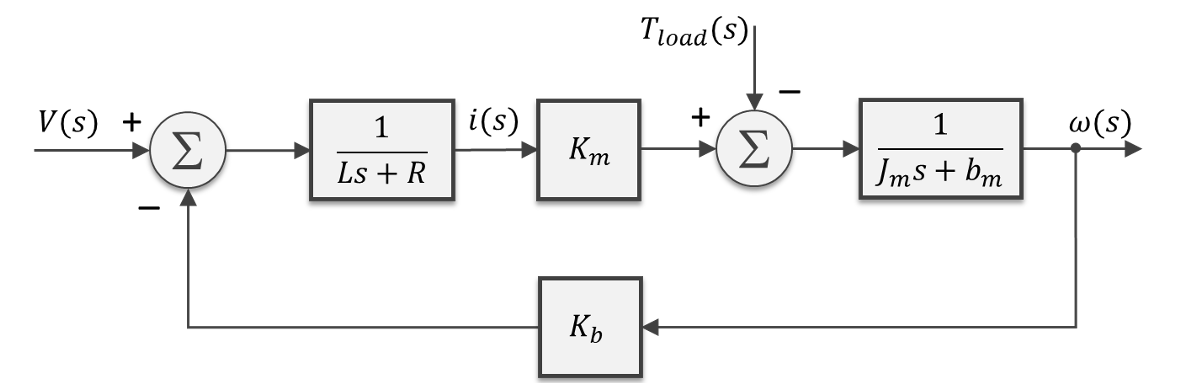
\includegraphics[width=0.8\columnwidth]{imgs/block diagram of the DC motor.png}
            \caption[Short description for list of figures]{The block diagram of the DC motor }
            \label{fig-magnitude}
            \end{figure}%

            Below is the Simulink drawing of the specified DC motor. In this model, terminal resistance, terminal inductance, back EMF constant, torque constant, rotor moment of inertia and mechanical friction coefficient specified as motor parameters in the data sheet are placed in the system. 5V is applied to the system as input voltage. In this structure; current, output voltage, output power, motor power, torque, motor speed, motor angle, load angle, load speed, counter torque and energy consumption are measured from the relevant points and collected via a 'bus selector' block and transferred to 'scope' blocks. Then, this data is connected to scope blocks and displayed graphically. Then, data is transferred to Matlab environment via 'to workspace' block; graphics are drawn here and added to the report.
            
    \begin{figure}[H]
        \centering
        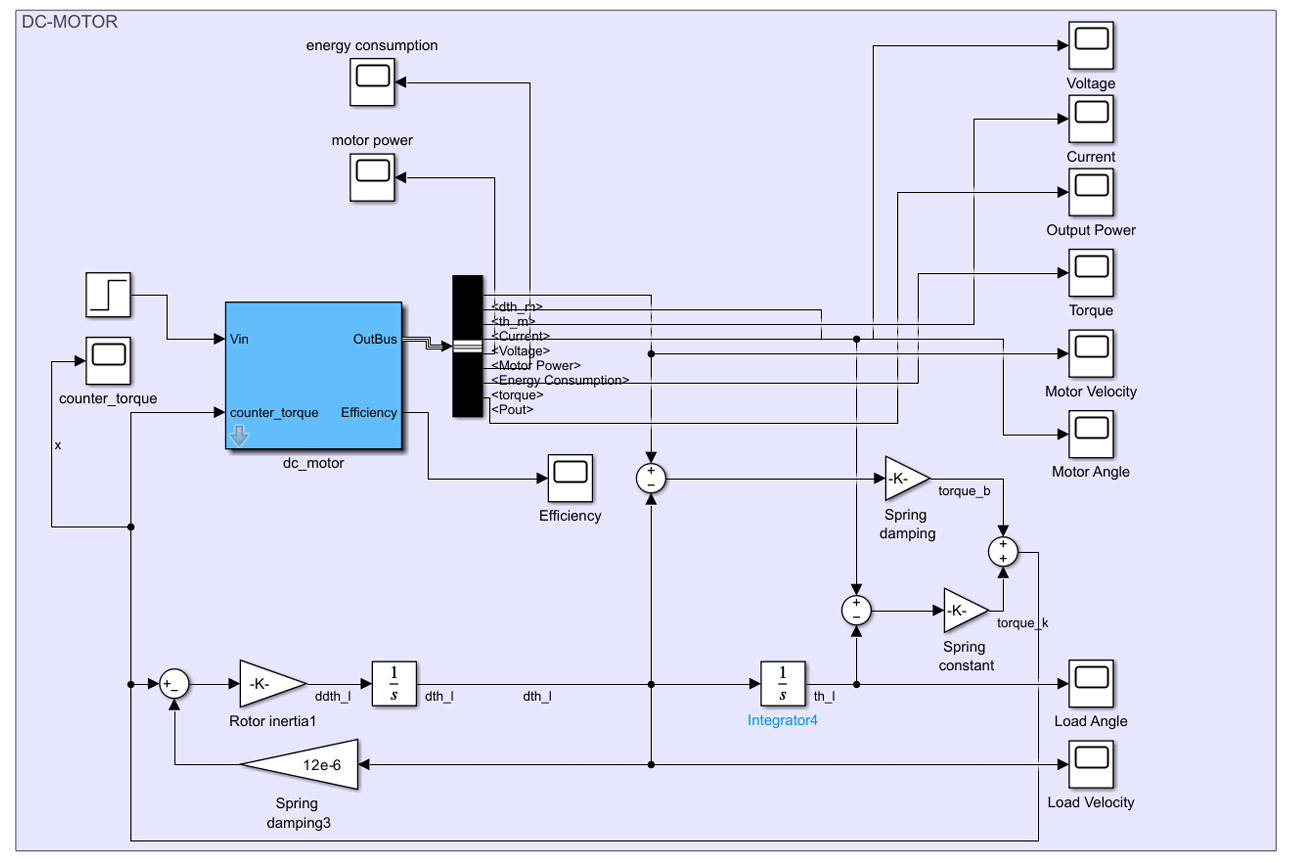
\includegraphics[width=0.8\columnwidth]{imgs/Simulink drawing of DC motor and load system.png}
        \caption[Short description for list of figures]{Simulink drawing of DC motor and load system }
        \label{fig-magnitude}
        \end{figure}%

        The internal structure of the subsystem (mask) block seen in blue above is as follows. Here, 
each parameter to be examined is connected to the outport port. 

\begin{figure}[H]
    \centering
    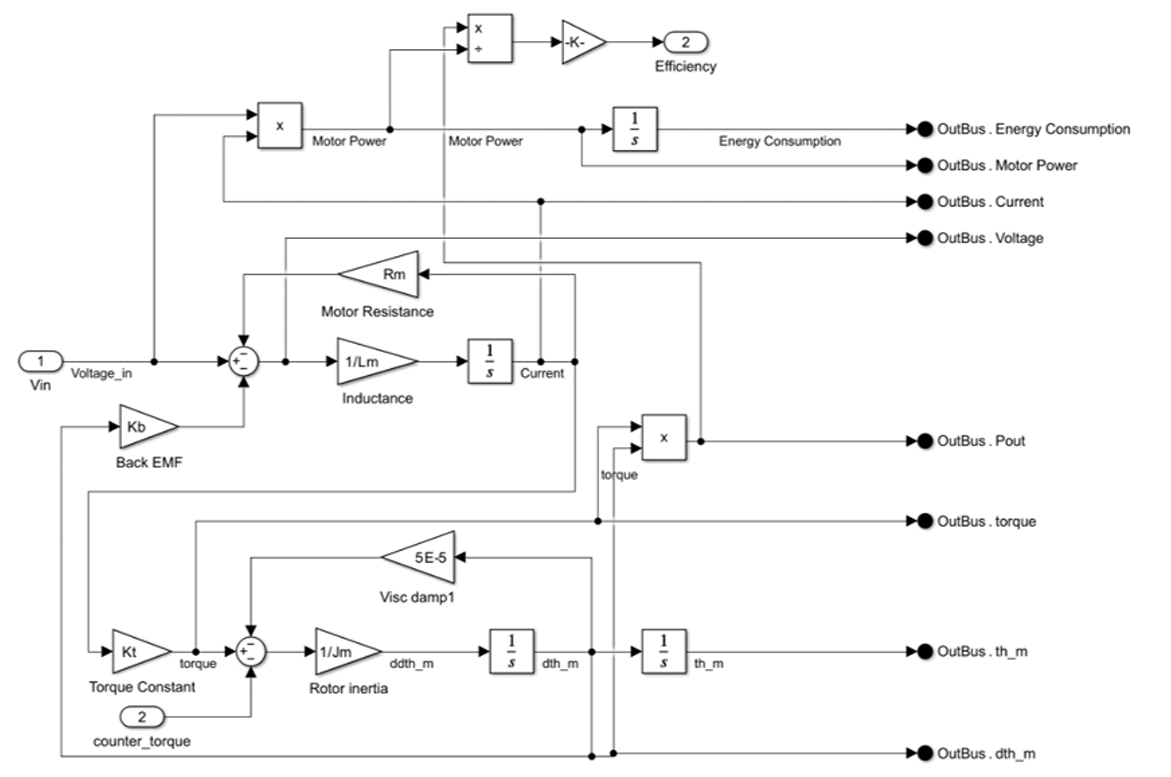
\includegraphics[width=0.8\columnwidth]{imgs/Tne inside of DC motor.png}
    \caption[Short description for list of figures]{Tne inside of DC motor }
    \label{fig-magnitude}
    \end{figure}%

    Detailed descriptions of the engine model and the corresponding graphical results are presented in Appendix B.

\section{dq Modeli ve Clarke–Park Dönüşümleri}

Üç fazlı elektrik makinelerinin analizi ve kontrolü, zamanla değişen üç fazlı ($a$-$b$-$c$) büyüklüklerin daha basit matematiksel modellerle ifade edilmesini gerektirir. Bu amaçla \textbf{Clarke} ve \textbf{Park} dönüşümleri kullanılır. Bu dönüşümler sayesinde, motorun $a$-$b$-$c$ sistemindeki karmaşık sinyalleri, durağan ($\alpha$–$\beta$) veya döner ($d$–$q$) referans sistemlerinde iki bağımsız bileşen ile temsil edilir. 

FOC (\textit{Field Oriented Control}) gibi gelişmiş kontrol stratejilerinde bu yöntemler, akı ve moment bileşenlerinin bağımsız kontrolünü mümkün kılar \cite{blashke1972,leonhard1996control}. dq modelinde motorun elektriksel dinamikleri, $d$ ve $q$ eksenlerine ait gerilim, akım ve akı bileşenleri üzerinden ifade edilir. Bu yaklaşım, asenkron motorun DC motor gibi kontrol edilmesine olanak sağlar \cite{macdonald1979dq}.

\subsection{Clarke Dönüşümü (abc $\rightarrow$ $\alpha\beta0$)}

Clarke dönüşümü, üç fazlı ($a$, $b$, $c$) dengeli sistemdeki akım veya gerilim bileşenlerini, $\alpha$-$\beta$ durağan eksen takımına ve sıfır bileşeni ($i_0$)’a dönüştürür. $\alpha$ ekseni genellikle $a$ fazı ile aynı doğrultuda alınır, $\beta$ ekseni ise ona dik olarak tanımlanır.

Dönüşüm matrisi:
\begin{equation}
\begin{bmatrix}
i_\alpha \\
i_\beta \\
i_0
\end{bmatrix}
=
\frac{2}{3}
\begin{bmatrix}
1 & -\frac{1}{2} & -\frac{1}{2} \\
0 & \frac{\sqrt{3}}{2} & -\frac{\sqrt{3}}{2} \\
\frac12 & \frac12 & \frac12
\end{bmatrix}
\begin{bmatrix}
i_a \\
i_b \\
i_c
\end{bmatrix}
\end{equation}

Burada:
\begin{itemize}
    \item $i_\alpha, i_\beta$: Durağan $\alpha$ ve $\beta$ eksenlerindeki bileşenler,
    \item $i_0$: Sıfır bileşeni (nötr akımı),
    \item $i_a, i_b, i_c$: Faz akımlarıdır.
\end{itemize}

Bu dönüşüm IEC 60034 standardında tanımlı üç fazlı ölçümler ile uyumludur ve sayısal kontrolörlerde (DSP, FPGA) gerçek zamanlı olarak hızlıca hesaplanabilir.

\subsection{Park Dönüşümü ($\alpha\beta$ $\rightarrow$ dq)}

Park dönüşümü, Clarke dönüşümü ile elde edilen $\alpha$-$\beta$ bileşenlerini, rotor akısına hizalanmış döner $d$-$q$ eksen takımına dönüştürür. $d$ ekseni akı bileşenini, $q$ ekseni ise moment bileşenini temsil eder.

\begin{equation}
\begin{bmatrix}
i_d \\
i_q \\
i_0
\end{bmatrix}
=
\begin{bmatrix}
\cos\theta & \sin\theta & 0 \\
-\sin\theta & \cos\theta & 0 \\
0 & 0 & 1
\end{bmatrix}
\begin{bmatrix}
i_\alpha \\
i_\beta \\
i_0
\end{bmatrix}
\end{equation}

Burada $\theta$, rotor akı vektörünün $\alpha$ ekseni ile yaptığı açıdır ve şu yöntemlerle bulunabilir:
\begin{itemize}
    \item Enkoder veya resolver gibi pozisyon sensörleri,
    \item Sensörsüz tahmin (MRAS, SMO, PLL tabanlı gözlemciler).
\end{itemize}

Bu dönüşüm sayesinde zamanla değişen AC sinyaller, sabit bileşenlere dönüşür ve PI kontrolörlerin etkin çalışması sağlanır. FOC algoritmalarında hassas tork ve akı kontrolü için kritiktir.

\subsection{dq Modelinin Matematiksel Temeli}

Bir asenkron motorun $dq$ eksenlerindeki gerilim denklemleri:
\begin{align}
v_d &= R_s i_d + \frac{d\psi_d}{dt} - \omega_e \psi_q \\
v_q &= R_s i_q + \frac{d\psi_q}{dt} + \omega_e \psi_d
\end{align}

Burada:
\begin{itemize}
    \item $v_d, v_q$: $d$ ve $q$ eksenlerindeki gerilimler,
    \item $i_d, i_q$: $d$ ve $q$ eksenlerindeki akımlar,
    \item $\psi_d, \psi_q$: $d$ ve $q$ eksenlerindeki akı bileşenleri,
    \item $R_s$: Stator direnci,
    \item $\omega_e$: Elektriksel açısal hızdır.
\end{itemize}

Elektromanyetik tork ifadesi:
\begin{equation}
T_e = \frac{3}{2} \cdot \frac{P}{2} \cdot (\psi_d i_q - \psi_q i_d)
\end{equation}

Bu ifade, $d$ ekseninde akı, $q$ ekseninde moment üretileceğini açıkça gösterir. $\psi_q$’nun sıfırlandığı alan yönlendirme koşulunda ($\psi_q = 0$), tork yalnızca $i_q$ akımıyla kontrol edilir.

\subsection{Standartlar ve Uygulama Notları}
dq modelinin pratikte uygulanabilmesi için motor parametrelerinin doğru ölçülmesi gerekir. Başlıca standartlar:
\begin{itemize}
    \item IEC 60034-2-1: Verim ölçüm metotları,
    \item IEC 60034-4: Senkron hız tespiti metotları,
    \item IEC 60034-12: Başlatma yöntemleri.
\end{itemize}

\textbf{Uygulama Notu:} $\theta$ açısındaki hata, akı ve moment bileşenlerinin karışmasına ve kontrol performansının bozulmasına yol açar. Bu nedenle yüksek hassasiyetli sensörler veya gelişmiş sensörsüz tahmin yöntemleri kullanılmalıdır \cite{macdonald1979dq}.

\begin{figure}[H]
    \centering
    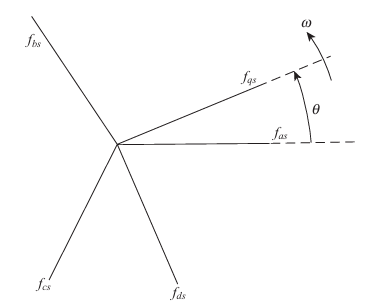
\includegraphics[width=0.75\linewidth]{imgs/dq_transformation.png}
    \caption{abc $\rightarrow$ $\alpha\beta$ $\rightarrow$ dq dönüşüm adımları}
    \label{fig:dq_transformation}
\end{figure}


\section{3 Fazlı 4 kW 4 Kutuplu WEG Motor} Örnek motor: WEG W22 IE3, 4 kW, 4 kutup, 50 Hz \begin{itemize} \item Senkron hız: $1500$ d/dk \item Nominal hız: $\approx 1450$ d/dk \item Gerilim: 220–240/380–415 V ($\Delta$/Y) \item Koruma sınıfı: IP55 \item Soğutma: IC411-TEFC \end{itemize} 

\section{FOC (Field Oriented Control)} FOC, stator akımını akı ($d$) ve tork ($q$) bileşenlerine ayırıp, bu iki bileşeni PI akım çevrimleri ile referanslarında tutarak hızlı ve hassas moment/hız kontrolü sağlar. Temel fikir, rotor akı vektörünü $d$ eksenine sabitlemek ve $q$ eksenini moment üretimi için kullanmaktır. 

\section{Verimlilik Hesabı} Motor verimi: \begin{equation} \eta = \frac{P_{out}}{P_{in}} = \frac{T \cdot \omega}{P_{in}} \end{equation} \begin{itemize} \item \textbf{Doğrudan yöntem:} Giriş gücü (üç faz güç analizörü) ve çıkış gücü (torkmetre + devir) ölçülerek hesaplanır. \item \textbf{Dolaylı yöntem:} Bakır, demir, mekanik ve ek kayıplar ölçülerek toplam kayıp bulunur ve giriş gücünden düşülür. \end{itemize} Ölçüm ve raporlama IEC 60034-2-1 standardına uygun yapılmalıdır.
 
\medskip




\clearpage
